\documentclass[]{article}
\usepackage[nomarkers, nolists]{endfloat}

%\linespread{1.6}
\usepackage{standalone}
\usepackage{amsmath}
\usepackage{amsfonts}
\usepackage{amsthm}
\usepackage[linktoc=all]{hyperref}
\usepackage[]{algorithm2e}
\usepackage{graphicx}
\usepackage{multirow}

\theoremstyle{plain}
\newtheorem{prop}{Proposition}
\theoremstyle{definition}
\newtheorem{defn}{Definition}
\newtheorem{exmp}{Example}
\theoremstyle{remark}
\newtheorem{rem}{Remark}

\title{Solving zero-dimensional polynomial systems:\\ a practical method using Bezout matrices}
\author{Jean-Paul Cardinal}

\begin{document}
\maketitle
\documentclass{standalone}
% Preamble
\begin{document}

\begin{abstract}
Let $f$ be a polynomial system consisting of $n$ polynomials $f_1,\cdots, f_n$ in $n$ variables $x_1,\cdots, x_n$, with coefficients in $\mathbb{Q}$ and let $\langle f\rangle$ be the ideal generated by $f$. Such a polynomial system, which has as many equations as variables is called a square system. It may be zero-dimensional, i.e the system of equations $f = 0$ has finitely many complex solutions, or equivalently the dimension of the quotient algebra $A = \mathbb{Q}[x]/\langle f\rangle$ is finite. In this case, the companion matrices of $f$ are defined as the matrices of the endomorphisms of $A$, called multiplication maps, $x_j : \left\vert
\begin{array}{c}
h \mapsto x_jh
\end{array}
\right.$, written in some basis of $A$.
We present a practical and efficient method to compute the companion matrices of $f$ in the case when the system is zero-dimensional. When it is not zero-dimensional, then the method works as well and still produces matrices having properties similar to the zero-dimensional case.
The whole method consists in matrix calculations. An experiment illustrates the method's effectiveness. 

\end{abstract}


\end{document}

\tableofcontents

%\documentclass{standalone}
% Preamble
\begin{document}

\section{Introduction}
The first step of this method is to construct the Bezout matrices associated to the ideal $I$. 
\end{document}

\documentclass{standalone}
% Preamble
\begin{document}

\section{Univariate case}
\label{univariate}
We recall some well-known facts about univariate polynomials;
in this section we consider a polynomial $f = a_0x^d + \dots + a_{d-1}x + a_d \in \mathbb{Q}[x]$ in the variable $x$, with rational coefficients; we denote by $A = \mathbb{Q}[x]/\langle f \rangle$ the quotient algebra of $\mathbb{Q}[x]$ by the ideal $\langle f \rangle$, and we denote indifferently by $x$ the variable $x$, its projection on the quotient algebra $A$ and the multiplication map $x : \left\vert h \mapsto xh \right.$ defined on $A$. 
The special basis $\bold{x} = (1, x,\cdots, x^{d-1})$ of the vector space $A$ is called the {\bf monomial basis}.

\subsection{Mutiplication maps}
The multiplication map $x : \left\vert h \mapsto xh \right.$ is an endomorphism of $A$ which, when written in the monomial basis, has a matrix $X$ called the {\bf companion matrix} of $f$. 
The matrix $X$ is Hessenberg and writes
\begin{equation}
\label{compan}
X =
\begin{bmatrix}
	0 & \cdots & 0 & -a_d/a_0 \\
	1 & 0 & \cdots & -a_{d-1}/a_0 \\
	\vdots  & \ddots  & \ddots & \vdots  \\
	0 & \cdots & 1 & -a_1/a_0
\end{bmatrix}
\end{equation}
\begin{prop}
\label{compan2roots}
The characteristic polynomial of $X$ is $f$.
\end{prop}

\begin{rem}
We deduce from Proposition \ref{compan2roots} that the eigenvalues of $X$ are the roots of $f$, taking account the multiplicities. 
Moreover, as the matrix $X$ is Hessenberg, we can use reliable techniques, like the QR algorithm, to compute its eigenvalues. 
This gives a practical and fast method to compute numerical approximations of the roots of $f$. 
\end{rem}

\begin{rem}
\label{g_1=g_2}
If $g_1, g_2$ are two polynomials of $\mathbb{Q}[x]$ that are equal modulo $f$, then $g_1(X) = g_2(X)$;
therefore, if $g \in A$, then the matrix $g(X)$ is defined without any ambiguity;
this matrix does not depend on the choice of the particular representative of $g$, and it is the matrix of the map $g:\left\vert h \mapsto gh \right.$, written in the monomial basis.
\end{rem}

\subsection{Bezout polynomials and Bezout matrices}
As we have seen, the companion matrix can be used to calculate the roots of a univariate polynomial. 
Interestingly, this can be naturally extended to zero-dimensional multivariate systems; 
if we have $n$ polynomials $f = f_1, \ldots, f_n$ in the variables $x = x_1, \ldots, x_n$, then we simply define the companion matrices as the matrices of the multiplication maps $x_j : \left\vert h \mapsto x_jh \right.$ defined on the quotient algebra $ A = \mathbb{Q}[x]/ \langle f\rangle$, written in some basis of $A$. 
However, in the multivariate case, $A$ has no canonical basis, and the companion matrices do not have an obvious form. 
We can nonetheless resolve this problem by using a family of matrices, the so-called Bezout matrices, that exists both in the univariate case and in the multivariate case, and that serve as intermediate matrices to construct the companion matrices. 
Let's introduce the Bezout matrices in the case of univariate polynomials.

\begin{defn}
\label{def_bez}
Let $f \in \mathbb{Q}[x]$ be a fixed polynomial. Let us introduce a new variable $y$ and let $g$ be any other polynomial. 
The {\bf Bezout polynomial} $\delta(g)$, or {\bf bezoutian}, is defined as the polynomial in the two variables $x, y$
$$
\delta(g) = \dfrac{f(x)g(y)-f(y)g(x)}{x-y}
$$
This polynomial is of degree $m-1$ in both variables $x, y$, where $m$ is the maximum of the degrees of $f$ and $g$.
If we write the bezoutian
\begin{equation}
\delta(g) = \sum_{\alpha,\beta = 0, \cdots, m-1} b_{\alpha\beta} x^\alpha y^\beta
\end{equation}
then the matrix of coefficients $B(g) = [b_{\alpha\beta}]$ is called the {\bf Bezout matrix}.
\end{defn}

\begin{rem}
The size of a Bezout matrix may be loosely defined; when working with several Bezout matrices, it may be desirable to pad some of them with extra columns or lines of zeros to get compatible sizes.
\end{rem}
\begin{rem}
The Bezout poynomial $\delta(g)$ and the Bezout matrix $B(g)$ satisfy the following equality
\begin{equation}
	\label{xBg}
	\delta(g) = \bold{x} B(g) \bold{y}^T
\end{equation}
with $\bold{x} = (1, x,\cdots, x^{m-1}) \in \mathbb{Q}[x]^m$ and $\bold{y} = (1, y,\cdots, y^{m-1}) \in \mathbb{Q}[y]^m$ are two vectors of monomials.
\end{rem}

\begin{exmp}
\label{exmp_1}
We choose $f = x^2 - 3x + 2$ as the fixed polynomial, and we examine the two cases $g=1$ and $g = x^3$. 
The Bezout polynomials are $\delta(1) = -3 + x + y$ and $\delta(x^3) = -2x^2 - 2xy -2y^2 + 3x^2y + 3xy^2 -x^2y^2$. 
The Bezout matrices $B(1)$ et $B(x^3)$ appear when we write  $\delta(1)$ and  $\delta(x^3)$ as double-entry arrays indexed by the monomials $1, x, x^2$ and $1, y, y^2$.
$$
\begin{array}{c|ccc}
\delta(1) & 1 & y & y^2\\
\hline
1 & -3 & 1 & 0\\
x & 1 & 0 & 0\\
x^2 & 0 & 0 & 0
\end{array}
\hspace{1cm}
\begin{array}{c|ccc}
\delta(x^3) & 1 & y & y^2\\
\hline
1 & 0 & 0 & -2\\
x & 0 & -2 & 3\\
x^2 & -2 & 3 & -1
\end{array}
$$
\end{exmp}

\begin{prop}
\label{relations_prop}
Let $f$ be a fixed polynomial and $g$ be another polynomial; if we denote by $m$ the maximum of the degrees of $f$ and $g$ and put $\bold{x} = (1, x,\cdots, x^{m-1})$, then
\begin{equation}
\label{relations}
	\bold{x}B(1)g = \bold{x}B(g)
\end{equation}
where the equality must be understood componentwise in $\mathbb{Q}[x]^m$ and modulo $f$.
\end{prop}
\begin{proof}
We rewrite $\delta(g)$ as
\begin{align*}
	\delta(g) & = & g(x)\dfrac{f(x)-f(y)}{x-y} - f(x)\dfrac{g(x)-g(y)}{x-y} \\ \nonumber
	\delta(g) & = & g(x)\delta(1) - f(x)\dfrac{g(x)-g(y)}{x-y}
\end{align*}
This equality holds between elements of $\mathbb{Q}[x][y]$. 
If $h\in \mathbb{Q}[x][y]$ and $\beta\in\mathbb{N}$, we denote by $h_\beta \in \mathbb{Q}[x]$ the coefficient of $y^\beta$ in the polynomial $h$; then
$$\delta(g)_\beta = g(x)\delta(1)_\beta - f(x)\left(\dfrac{g(x)-g(y)}{x-y}\right)_\beta$$
which holds in $\mathbb{Q}[x]$. Thus, we have $\delta(g)_\beta = g(x)\delta(1)_\beta$ modulo $f$; as this is true for all $\beta\in\mathbb{N}$, Equality (\ref{relations}) follows.
\end{proof}

\begin{rem}
Each column of a Bezout matrix, when left-multiplied by $\bold{x}$, is a polynomial in the variable $x$; when this does not bring to confusion, we will think of columns of a Bezout matrix as elements of $\mathbb{Q}[x]$, and lines as elements of $\mathbb{Q}[y]$.
Saying Proposition \ref{relations_prop} differently : each column of $B(1)$, when multiplied by $g$, equals the column of same index of $B(g)$, modulo $f$.
\end{rem}

\begin{exmp}
Returning to Example \ref{exmp_1}, Proposition \ref{relations_prop} says that the following equalities hold, modulo $f$
\begin{align*}
 (-3 + x)x^3 &= -2x^2, \\
 (1)x^3 &= -2x + 3x^2, \\
 (0)x^3 &= -2 + 3x - x^2
\end{align*}
\end{exmp}

\begin{rem}
If we work with lines instead of columns, then Proposition \ref{relations_prop} says that $gB(1)\bold{y}^T = B(g)\bold{y}^T$, giving equalities in $\mathbb{Q}[y]/\langle f \rangle$.
\end{rem}


\subsection{Relation between Bezout matrices and the companion matrix}
\label{Bar}
Given a fixed polynomial $f$ of degree $d$, the bezoutians $\delta(1)$ and $\delta(x)$ write
\begin{equation}
	\begin{array}{c|cccc}
		\delta(1) & 1 & y & \dots & y^{d-1} \\
		\hline
		1 & a_{d-1} & \ldots & \dots & a_0 \\
		x & a_{d-2} & \dots & a_0 & 0 \\
		\vdots & \vdots & \vdots & \vdots & \vdots \\
		x_{d-1} & a_0 & 0 & \ldots & 0 \\
	\end{array}
	\hspace{1.5cm}
	\begin{array}{c|cccc}
		\delta(x) & 1 & y & \dots & y^{d-1} \\
		\hline
		1 & -a_{d} & 0 & \dots & 0 \\
		x & 0 & a_{d-2} & \ldots & a_0 \\
		\vdots & \vdots & \vdots & \vdots & \vdots \\
		x_{d-1} & 0 & a_0 & \ldots & 0 \\
	\end{array}.
\end{equation}
The corresponding arrays of coefficients are the Bezout matrices $B(1)$, which is clearly invertible, and $B(x)$. 
These two matrices are specially important because they are related to the companion matrix:
\begin{prop}
\label{Barnett}
The compagnon matrix $X$ and the Bezout matrices $B(x), B(1)$ are related by the {\bf Barnett decomposition} formula
\cite{Barnett}
\begin{equation}
	X = B(x)B(1)^{-1}
\end{equation}
\end{prop}

\begin{proof}
Let us consider the two families of elements of the quotient algebra $A$
\begin{equation}
	\begin{array}{lll}
		\bold{x}B(1) & = & (a_{d-1} + a_{d-2}x + \cdots + a_0x^{d-1}, \cdots, a_1 + a_0x,  a_0).\\
		\bold{x}B(x) & = & (-a_d, a_{d-2}x + \cdots + a_0x^{d-1}, \cdots, a_0x)
	\end{array}
\end{equation}
and put $\hat{\bold{x}} = \bold{x}B(1)$.
As $B(1)$ is invertible, the family $\hat{\bold{x}}$ is a basis of the vector space $A$, called the {\bf Horner basis}.
From Proposition \ref{relations_prop}, we have $\hat{\bold{x}}x = \bold{x}B(1)$. 
By construction, $B(1)$ is the matrix of the Horner basis $\hat{\bold{x}}$ written on the monomial basis $\bold{x}$, and $B(x)$ is the matrix of the family $\hat{\bold{x}}x$ written on the monomial basis;
$B(1)^{-1}B(x)$ is thus the matrix of the family $\hat{\bold{x}}x$ written on the Horner basis $\hat{\bold{x}}$. 
This means that the multiplication map $x : \left\vert h \mapsto xh\right.$ is represented in the Horner basis $\hat{\bold{x}}$ by the matrix $B(1)^{-1}B(x)$;
the multiplication map $x$ is also represented in the monomial basis $\bold{x}$ by the matrix $B(1)(B(1)^{-1}B(x))B(1)^{-1} = B(x)B(1)^{-1}$.
\end{proof}

\subsection{Barnett decomposition formula}
\label{Bar_gen}
The Barnett decomposition formula relates the companion matrix, representing the multiplication map $x$, to the Bezout matrices of the polynomials $1$ and $x$;
this can be naturally extended as follows.
Let $g \in \mathbb{Q}[x]$ be any polynomial;
the Bezout matrices $B(1)$ et $B(g)$ are related to the matrix $g(X)$ by the {\bf general Barnett decomposition formula}
\begin{equation}
	\label{GBG}
	B(g)B(1)^{-1} = g(X)
\end{equation}
given that if the sizes of $B(1)$ and $B(g)$ differ, then we must transform and resize $B(g)$ according to a procedure that we shall now explain on the following example.

Formula~(\ref{GBG}) is easily checked when the degree of $g$ is smaller or equal to the degree of $f$, because $B(1)$ and $B(g)$ have the same size;
for example, if $f = x^2 - 3x + 2$, then we have
$$
\begin{array}{c|cc}
	\delta(1) & 1 & y \\
	\hline
	1 & -3 & 1 \\
	x & 1 & 0
\end{array}
\hspace{1cm}
\begin{array}{c|cc}
	\delta(x) & 1 & y \\
	\hline
	1 & -2 & 1 \\
	x & 1 & 0
\end{array}
\hspace{1cm}
\begin{array}{c|cc}
	\delta(x^2) & 1 & y \\
	\hline
	1 & 0 & -2 \\
	x & -2 & 3
\end{array}
$$
and
\begin{equation}
	B(x)B(1)^{-1} =
	\begin{bmatrix}
		0 & -2 \\
		1 & 3
	\end{bmatrix}
	= X
	\hspace{1cm}
	B(x^2)B(1)^{-1} =
	\begin{bmatrix}
		-3 & -6 \\
		2 & 7
	\end{bmatrix}
	= X^2
\end{equation}
which is consistent with formula~(\ref{GBG}).
On the other hand, if $m$, the degree of $g$ is strictly larger than $d$, the degree of $f$, then the sizes of $B(g)$ and $B(1)$ differ, and the product $B(g)B(1)^{-1}$ no longer makes sense. 
This can be fixed by indexing the Bezout matrices by the same monomials, namely $\bold{x} = (1, x,\cdots, x^{m-1})$ and $\bold{y} = (1, y,\cdots, y^{m-1})$. 
For example, with $f$ as above and $g = x^3$, we have
$$
\begin{array}{c|ccc}
\delta(1) & 1 & y & y^2\\
\hline
1 & -3 & 1 & 0\\
x & 1 & 0 & 0\\
x^2 & 0 & 0 & 0
\end{array}
\hspace{1cm}
\begin{array}{c|ccc}
\delta(x^3) & 1 & y & y^2\\
\hline
1 & 0 & 0 & -2\\
x & 0 & -2 & 3\\
x^2 & -2 & 3 & -1
\end{array}
$$
In doing so, $B(1)$ is no longer invertible;
the key to obtain simultaneously matrices of equal size and the invertibility of $B(1)$, is to reduce the bezoutians modulo $f$. 
Let's illustrate this process on the previous example, and write
\begin{align} \nonumber %%%%%%%%%%%%%%
	\delta(x^3) &=
	\begin{bmatrix}
			1 & x & x^2
	\end{bmatrix}
	\begin{bmatrix}
		0 & 0 & -2 \\
		0 & -2 & 3 \\
		-2 & 3 & -1
	\end{bmatrix}
	\begin{bmatrix}
		1 \\
		y \\
		y^2
	\end{bmatrix} \\ \nonumber %%%%%%%%%%%%%%
	\delta(x^3) &=
	\begin{bmatrix}
		1 & x & x^2
	\end{bmatrix}
	\begin{bmatrix}
		1 & 0 & 2 \\
		0 & 1 & -3 \\
		0 & 0 & 1
	\end{bmatrix}
	\begin{bmatrix}
		1 & 0 & -2 \\
		0 & 1 & 3 \\
		0 & 0 & 1
	\end{bmatrix}
	\begin{bmatrix}
		0 & 0 & -2 \\
		0 & -2 & 3 \\
		-2 & 3 & -1
	\end{bmatrix}
	\begin{bmatrix}
		1 \\
		y \\
		y^2
	\end{bmatrix} \\ \nonumber %%%%%%%%%%%%%%%
	\delta(x^3) &=
	\begin{bmatrix}
			1 & x & 2 - 3x + x^2
	\end{bmatrix}
	\begin{bmatrix}
		4 & -6 & 0 \\
		-6 & 7 & 0 \\
		-2 & 3 & -1
	\end{bmatrix}
	\begin{bmatrix}
		1 \\
		y \\
		y^2
	\end{bmatrix} \\ \nonumber %%%%%%%%%%%%%%
\end{align}
To sum up, we have post-multiplied the row vector
$\begin{bmatrix}
	1 & x & x^2
\end{bmatrix}$ by the Gauss transform
$$P =
\begin{bmatrix}
	1 & 0 & 2 \\
	0 & 1 & -3 \\
	0 & 0 & 1
\end{bmatrix}$$
and pre-multiplied the two Bezout matrices $B(1)$ and $B(g)$ by $P^{-1}$. The bezoutians now write
$$
\begin{array}{c|ccc}
	\delta(1) & 1 & y & y^2\\
	\hline
	1 & -3 & 1 & 0\\
	x & 1 & 0 & 0\\
	2 - 3x + x^2 & 0 & 0 & 0
\end{array}
\hspace{1cm}
\begin{array}{c|ccc}
	\delta(x^3) & 1 & y & y^2\\
	\hline
	1 & 4 & -6 & 0 \\
	x & -6 & 7 & 0 \\
	2 - 3x + x^2 & -2 & 3 & -1
\end{array}
$$
According to the relations~(\ref{relations}) the third column of $\delta(x^3)$,  $-2 + 3x - x^2$, is zero modulo $f$; we recognize the simple fact $-f = 0$. Thus,
\begin{align} \nonumber %%%%%%%%%%%%%%
\delta(1) &= \begin{bmatrix}
	1 & x
\end{bmatrix}
\begin{bmatrix}
	-3 & 1 \\
	1 & 0
\end{bmatrix} \nonumber %%%%%%%%%%%%%%
\begin{bmatrix}
	1 \\
	y
\end{bmatrix}\\
\delta(x^3) &= \begin{bmatrix}
	1 & x
\end{bmatrix}
\begin{bmatrix}
	4 & -6 \\
	-6 & 7
\end{bmatrix} \nonumber %%%%%%%%%%%%%%
\begin{bmatrix}
	1 \\
	y
\end{bmatrix} + (2 - 3x + x^2)(-2 + 3y - y^2)
\end{align}
Now, the bezoutians, when reduced modulo $f$ write
$$
\begin{array}{c|cc}
	\delta(1) & 1 & y \\
	\hline
	1 & -3 & 1 \\
	x & 1 & 0
\end{array}
\hspace{1cm}
\begin{array}{c|cc}
	\delta(x^3) & 1 & y \\
	\hline
	1 & 4 & -6  \\
	x & -6 & 7
\end{array}
$$
We have obtained two Bezout matrices of equal size, with $B(1)$ invertible. 
If we compute the matrix ratio
\begin{equation}
	B(x^3)B(1)^{-1} =
	\begin{bmatrix}
		-6 & -14 \\
		7 & 15
	\end{bmatrix}
	= X^3
\end{equation}
then we see that it is consistent with the general Barnett decomposition formula~(\ref{GBG}).

\begin{rem}
Instead of a Gauss matrix, we may use any matrix that maps a given column vector to a column vector containing just one non-zero entry, such as, for example, a Householder orthogonal matrix. This is the choice made in the implementation of the practical method given in \cite{jp_code}.

\end{rem}

\end{document}

%%% Local Variables:
%%% mode: latex
%%% TeX-master: "bezout"
%%% End:

\documentclass{standalone}
% Preamble
\begin{document}


\section{Multivariate case}
\label{multivariate}

For a univariate polynomial $f$, the structure of the quotient algebra $A$ consists of the monomial basis and the companion matrix; this matrix is obtained either by a direct reading of the coefficients of $f$, or by taking the ratio of the two matrices $B(1), B(x)$; in contrast, for a multivariate polynomial system, neither a basis nor the companion matrices (matrices of the multiplication maps
$x_j : \left\vert
\begin{array}{c}
h \mapsto x_jh
\end{array}
\right.$ in the basis) can be read from the coefficients of the given polynomials. It is easy, however, to construct the Bezout matrices $B(1), B(x_1), \cdots, B(x_n)$, from which one can derive a basis of $A$ and the related companion matrices $X_1,\cdots, X_n$. 
Let's set the framework: given $n$ polynomials $f_1,\cdots, f_n$ in the variables $x_1,\cdots, x_n$, with coefficients in $\mathbb{Q}$, we denote by
\begin{itemize}
\item $\mathbb{Q}[x]$ the ring of polynomials in the variables $x = x_1,\cdots, x_n$,
\item $\langle f \rangle$ the idal generated by $f = f_1,\cdots, f_n$,
\item $A = \mathbb{Q}[x]/\langle f\rangle$ the quotient algebra.
\end{itemize}
From now on we assume that $\langle f\rangle$ is {\bf zero-dimensional}, that is to say the vector space $A$ is finite dimensional \cite[p.~234]{clo}. This is always the case when $n = 1$.

\subsection{Construction of Bezout polynomials and Bezout matrices}

\subsubsection{Extension of Definition \ref{def_bez} to the multivariate case}

\begin{defn}
Let $x^\gamma = x_1^{\gamma_1}\cdots x_n^{\gamma_n} \in \mathbb{Q}[x]$ be some monomial.
We introduce a new variable set $y = y_1,\cdots, y_n$ and consider, for each couple of indices $i, j = 1\cdots n$, the ratio
\begin{equation}
\label{finite_diff}
\delta_{i,j}(x^\gamma) = \dfrac{y_j^{\gamma_j}f_i(y_1,\cdots, y_{j-1},x_j,\cdots,x_n) - x_j^{\gamma_j}f_i(y_1,\cdots,y_j,x_{j+1},\cdots,x_n)}{x_j - y_j}
\end{equation}
which is a polynomial in the variables $x, y$. 
With the $\delta_{i,j}$'s we form a finite difference matrix
\begin{equation}
\label{Delta}
\Delta(x^\gamma) = (\delta_{ij}(x^\gamma))_{ij}
\end{equation}
whose determinant $\delta(x^\gamma) = det(\Delta(x^\gamma))$, a polynomial in both variables $x, y$, is called the {\bf Bezout polynomial}, or {\bf bezoutian}, of $x^\gamma$.
This definition can be extended by linearity to a more general polynomial $g = \sum_\gamma g_\gamma x^\gamma \in \mathbb{Q}[x]$ by the formula
$$\delta(g) = \sum_\gamma g_\gamma \delta(x^\gamma)$$
Writting $\delta(g)$ as a sum of monomials, 
\begin{equation}
\label{def_bez}
\delta(g) = \sum_{0 \le \alpha,\beta} b_{\alpha\beta} x^\alpha y^\beta
\end{equation} 
we define $B(g)$, the {\bf Bezout matrix} of $g$, as the matrix of the coefficients $B(g) = [b_{\alpha\beta}]$. If we denote by $\bold{x}$ and $\bold{y}$ the sets of all the monomials $x^\alpha$ et $y^\beta$ that appear in~(\ref{def_bez}), then we have the relation, similar to~(\ref{xBg})
\begin{equation}
	\delta(g) = \bold{x} B(g) \bold{y}^T
\end{equation}
\end{defn}
The following example, see \cite{jpc}, illustrates the previous definitions

\begin{exmp}
\label{bez_multi}
We take $n = 2$, $f_1 = x_1^2 + x_1x_2^2 - 1, f_2 = x_1^2x_2 + x_1$ and want to calculate the Bezout matrices $B(1), B(x_1), B(x_2)$, which are useful for computing the companion matrices $X_1, X_2$. To begin with, we compute the finite difference matrices, as defined in (\ref{Delta})
\begin{align}
\Delta(1) &=
\begin{pmatrix}
x_1 + x_2^2 + y_1 & x_2y_1 + y_1y_2 \\
1 + x_1x_2 + x_2y_1 & y_1^2
\end{pmatrix} \nonumber  \\
\Delta(x_1) &=
\begin{pmatrix}
1 + x_1y_1 & x_2y_1 + y_1y_2 \\
1 + x_1x_2 + x_2y_1 & y_1^2
\end{pmatrix} \nonumber  \\
\Delta(x_2) &=
\begin{pmatrix}
x_1 + x_2^2 + y_1 & 1 - y_1^2 + x_2y_1y_2 \\
1 + x_1x_2 + x_2y_1  & -y_1
\end{pmatrix} \nonumber
\end{align}
whose determinants are the bezoutians
\begin{align}
\delta(1) &= -x_2y_1 - x_1x_2^2y_1 + x_1y_1^2 + y_1^3 - y_1y_2 - x_1x_2y_1y_2 - x_2y_1^2y_2 \nonumber \\
\delta(x_1) &=  y_1^2 - x_1x_2^2y_1^2 + x_1y_1^3 - x_1x_2y_1^2y_2 \nonumber \\
\delta(x_2) &= -1 - x_1x_2 - x_1y_1 -x_2y_1 - x_2^2y_1 + x_1x_2y_1^2 + x_2y_1^3 - x_2y_1y_2 - x_1x_2^2y_1y_2 - x_2^2y_1^2y_2\nonumber
\end{align}
The monomial appearing in these polynomials are
$\bold{x} = (1, x_2, x_2^2, x_1, x_1x_2, x_1x_2^2)$ and $\bold{y} = (1, y_1, y_1y_2, y_1^2, y_1^2y_2, y_1^3)$; the Bezout matrices $B(1), B(x_1), B(x_2)$ appear when we write these bezoutians as double-entry arrays indexed by $\bold{x}, \bold{y}$
$$\begin{array}{c|cccccc}
	\delta(1) & 1 & y_1 & y_1y_2 & y_1^2 & y_1^2y_2 & y_1^3 \\
	\hline
	1 &  &  & -1 &  &  & 1\\
	x_2 &  & -1 &  &  & -1 & \\
	x_2^2 &  &  &  &  &  & \\
	x_1 &  &  &  & 1 &  & \\
	x_1x_2 &  &  & -1 &  &  & \\
	x_1x_2^2 &  & -1 &  &  &  &
\end{array}$$
$$\begin{array}{c|cccccc}
	\delta(x_1) & 1 & y_1 & y_1y_2 & y_1^2 & y_1^2y_2 & y_1^3 \\
	\hline
	1 &  &  &  & 1 &  & \\
	x_2 &  &  &  &  &  & \\
	x_2^2 &  &  &  &  &  & \\
	x_1 &  &  &  &  &  & 1\\
	x_1x_2 &  &  &  &  & -1 & \\
	x_1x_2^2 &  &  &  & -1 &  &
\end{array}$$
$$\begin{array}{c|cccccc}
	\delta(x_2) & 1 & y_1 & y_1y_2 & y_1^2 & y_1^2y_2 & y_1^3 \\
	\hline
	1 & -1 &  &  &  &  & \\
	x_2 &  & -1 & -1 &  &  & 1\\
	x_2^2 &  & -1 &  &  & -1 & \\
	x_1 &  & -1 &  &  &  & \\
	x_1x_2 & -1 &  &  & 1 &  & \\
	x_1x_2^2 &  &  & -1 &  &  &
\end{array}$$

\end{exmp}

\begin{rem}
Contrasting with the univariate case, $\bold{x}$ and $\bold{y}$ are not bases of the vector space $A$. 
But, as we will see, they are  generating sets and we will examine how to build bases from them.
\end{rem}

\subsubsection{Practical computation of the Bezout matrices}
In the previous example, the matrices $\Delta(1), \Delta(x_1), \Delta(x_2)$ have size $2$ and their entries are polynomials in $x_1, x_2$; calculating their determinant is easy. But, if either the number  $n$ of variables or the degree of the input polynomials $f_i$ increase, then this calculation becomes impractical because one cannot use the Gauss pivot algorithm to a polynomial entries matrix. We can however overcome this difficulty by applying the following evaluation-interpolation process :
\begin{enumerate}
\item
Estimate a priori the set of monomials $x^\alpha y^\beta$ appearing in the Bezout polynomial $\delta(x_k)$ (for fixed $k$, $k = 0,\cdots, n$, with the convention that $x_0 = 1$). Specifically, if we suppose that the polynomial system $f$ has multi-degree $(d_1, \cdots, d_n)$, that is to say, the partial degree in the variable $x_j$ of each $f_i$ is smaller or equal to $d_j$,then the polynomial $\delta(x_k)$ has multi-degree $(d_1, 2d_2, \cdots, nd_n)$ in variable $x$ and multi-degree $(nd_1, (n-1)d_2, \cdots, d_n)$ in variable $y$. Note that this estimate is the same for each $k$.
\item
Evaluate the polynomial-entries matrix $\Delta(x_k)$ on all pairs $(u, v)$ where $u = (u_1,\cdots, u_n) \in U$ and $v = (v_1,\cdots, v_n) \in V$, $U, V$ being adequate sets of Fourier multi-points. We can choose, for instance, $U = \prod_{j=1..n} U_j$ where $U_j$ is the set of complex roots of the polynomial $X^{jd_j} - 1$; and we must choose $V = \prod_{j=1..n} V_j$ in such a way that $U_j$ et $V_j$ are disjoint sets, so that the denominator of the ratio (\ref{finite_diff}) never vanishes. This is obtained, for example, if $V_j$ is the set of complex roots of the polynomial $X^{(n-j+1)d_j} - \theta_j$ with $\theta_j = e^{i\pi/j}$ (here $i$ means the square root of $-1$). 
\item
For each $(u, v) \in U\times V$, apply the Gauss pivot method to the numerical matrix $\Delta(x_k)(u, v)$ in order to compute its determinant $\delta(x_k)(u, v)$. This produces a matrix $C^{(k)}$ defined by $C^{(k)}_{u, v} = \delta(x_k)(u, v)$.
\item
Interpolate the set of numerical values $\delta(x_k)(u, v)$ in order to obtain the Bezout polynomial $\delta(x_k)$ and the Bezout matrix $B^{(k)}$.
\end{enumerate}

These considerations lead to the following algorithm providing the sets $U$ and $V$.
\begin{algorithm}[]
\label{fourierPoints}
\KwData{$d = (d_1, \cdots, d_n)$, multi-degree of polynomial system}
\KwResult{$U, V$, two sets of Fourier points}
\For{$j = 1,\cdots, n$}{
	$U_j \gets$ roots of $X^{jd_j}-1$\;
	$V_j \gets$ roots of $X^{(n-j+1)d_j}-e^{i\pi/j}$\;
}
$U \gets \prod_{j=1..n}U_j$\;
$V \gets \prod_{j=1..n}V_j$\;
\caption{Construction of $U, V$, two sets of Fourier points}
\end{algorithm}

Then, we evaluate the bezoutian $\delta(x_k)$ on the Fourier points $(u, v) \in U\times V$

\begin{algorithm}[]
\label{algo_2}
\KwData{polynomial sytem $f$, index $k$}
\KwResult{matrix $C^{(k)}$ containing the evaluations $\delta(x_k)(u, v)$}
$(d_1, \cdots, d_n) \gets$ multi-degree of $f$\;
Get $U, V$ via Algorithm \ref{fourierPoints}\;
$D \gets \prod_{j=1..n}jd_j$\;
$C^{(k)} \gets \textsc{zeros}(D, D)$\;
\For{$(u, v) \in U\times V$}{
	$\Delta \gets \textsc{zeros}(n, n)$\;
	\For{$i, j=1..n$}{
		$\Delta_{i,j} \gets \delta_{i,j}(x_k)(u, v)$
	}
	$C^{(k)}_{u, v} \gets \textsc{det}(\Delta)$
}
\caption{Evaluation of the bezoutian $\delta(x_k)$ on $U\times V$}
\end{algorithm}

Let us show, to conclude, how the Bezout matrix $B(x_k)$ is simply related to $C^{(k)}$.
To simplify, we denote the bezoutian $\delta(x_k)$ by $\delta^{(k)}$ and the Bezout matrix $B(x_k)$ by $B^{(k)}$; recall that $C^{(k)}$ denotes the evaluation matrix of $\delta^(k)$ on $U\times V$.
The matrix $B^{(k)} = \left[b^{(k)}_{\alpha\beta}\right]$ satisfies $\delta^{(k)}(x, y) = \sum_{\alpha,\beta} b^{(k)}_{\alpha\beta} x^\alpha y^\beta$,
thus $C^{(k)}_{u,v} = \delta^{(k)}(u, v) = \sum_{\alpha,\beta} b^{(k)}_{\alpha\beta} u^\alpha v^\beta$; this writes as a matrix product
$\left[C^{(k)}_{u,v}\right]_{u,v} = \left[u^\alpha\right]_{u,\alpha} \left[b^{(k)}_{\alpha,\beta}\right]_{\alpha, \beta} \left[v^\beta\right]_{v, \beta}^T$. If we define the Fourier matrices $F_u = \left[ u^\alpha \right]_{u, \alpha}$ and $F_v = \left[ v^\beta \right]_{v, \beta}$, then we get the evaluation-interpolation relation between matrices $B^{(k)}$ and $C^{(k)}$
\begin{equation}
C^{(k)} = F_uB^{(k)} F_v^T
 \end{equation}
Since $U$ and $V$ consist of Fourier points, $F_u$ et $F_v$ are unitary and $B^{(k)}$ writes as the matrix product
 \begin{equation}
 B^{(k)} = F_u^*C^{(k)} \overline{F_v}
 \end{equation}
The computation of the Bezout matrices, as described above, have been implemented in Numpy and can be found at \cite{jp_code}.

\end{document}

\documentclass{standalone}
% Preamble
\begin{document}


\subsection{Barnett decomposition formula and structure of the quotient algebra.}
Since the ideal $\langle f\rangle$ is zero-dimensional, the dimension of the quotient algebra $A = \mathbb{Q}[\bold{x}]/\langle f\rangle$ is finite; we may look for some basis and its related companion matrices (matrices of the multiplication maps by $x_1,\cdots, x_n$). 
For this purpose, we will adapt the process described in Section \ref{Bar_gen} but, before, we will specify a number of algebraic properties about the polynomial $\delta^0$ and matrices $B^{(k)}$.
\subsubsection{Algebraic properties of polynomial $\delta^0$ and matrix $B^{(0)}$}
The following properties are simple; for a proof, the interested reader may refer to \cite{jpc}. As in Proposition \ref{Barnett}, we define families of elements of $A$ by forming the vector-matrix products
\begin{equation}
		\hat{\bold{x}}_k  =  \bold{x}B^{(k)}, \quad k=0\cdots n
\end{equation}
with the convention that $x_0=1$ and where $\bold{x}$ is the set of all the monomials $x^\alpha$ appearing in the Bezout polynomials $\delta^{(k)}, \quad k=0\cdots n$. We also write $\hat{\bold{x}}_0 = \hat{\bold{x}}$.
\begin{exmp}
Following Example \ref{bez_multi} we have
\begin{equation}
	\begin{array}{lll}
		\hat{\bold{x}} & = & (0, -x_2 - x_1x_2^2, -1 - x_1x_2, x_1, -x_2, 1) \\
		\hat{\bold{x}}_1 & = & (0, 0, 0, -1 - x_2^2, -x_1x_2, x_1) \\
		\hat{\bold{x}}_2 & = & (-1 - x_1x_2, -x_2 - x_2^2 - x_1, - x_2 - x_1x_2^2, x_1x_2, -x_2^2, x_2)
	\end{array}
\end{equation}
\end{exmp}

\begin{prop}
\label{xj} (see \cite{jpc}).
For all $k=1\cdots n$ we have
\begin{equation}
    \hat{\bold{x}}x_k = \hat{\bold{x}}_k
\end{equation}
\end{prop}
This proposition can be easily checked on Example \ref{bez_multi}. 
So far, the univariate and multivariate cases are very similar, except on one point : in the multivariate case the families $\bold{x}$ and $\hat{\bold{x}}$ are not, in general, bases of the vector space $A$. We have, however, the weaker result (see \cite{jpc}) :

\begin{prop}
Both $\bold{x}$ and $\hat{\bold{x}}$ are generating families of the vector space $A$.
\end{prop}

\subsubsection{Reduction process}
\label{sec:reduction_process}
Following the matrix handlings described in Section \ref{Bar_gen}, we now show how to compute, starting from the generating families $\bold{x}, \hat{\bold{x}}$ and the Bezout matrices $B^{(k)}$, a basis of $A$ and the companion matrices $X_k$.
Let us illustrate this process on Example \ref{bez_multi}.\\
The first column of $B^{(0)}$ is zero but that of de $B^{(2)}$ is not; this gives the relation $1 + x_1x_2 = 0$, modulo $I$. Then, we right-multiply $\bold{x}$ by the Gauss matrix $P$ whose $5$th column is $(1, 0, 0, 0, 1, 0)^{T}$ and left-multiply the Bezout matrices by $P^{-1}$; the Bezout polynomials write 
$$
\begin{array}{c|cccccc}
	\delta^{(0)} & 1 & y_1 & y_1y_2 & y_1^2 & y_1^2y_2 & y_1^3 \\
	\hline
	1 &  &  &  &  &  & 1\\
	x_2 &  & -1 &  &  & -1 & \\
	x_2^2 &  &  &  &  &  & \\
	x_1 &  &  &  & 1 &  & \\
	1+x_1x_2 &  &  & -1 &  &  & \\
	x_1x_2^2 &  & -1 &  &  &  &
\end{array}$$
$$
\begin{array}{c|cccccc}
	\delta^{(1)} & 1 & y_1 & y_1y_2 & y_1^2 & y_1^2y_2 & y_1^3 \\
	\hline
	1 &  &  &  & 1 & 1 & \\
	x_2 &  &  &  &  &  & \\
	x_2^2 &  &  &  &  &  & \\
	x_1 &  &  &  &  &  & 1\\
	1+x_1x_2 &  &  &  &  & -1 & \\
	x_1x_2^2 &  &  &  & -1 &  &
\end{array}
\hspace{0.2cm}
\begin{array}{c|cccccc}
	\delta^{(2)} & 1 & y_1 & y_1y_2 & y_1^2 & y_1^2y_2 & y_1^3 \\
	\hline
	1 &  &  &  & -1 &  & \\
	x_2 &  & -1 & -1 &  &  & 1\\
	x_2^2 &  & -1 &  &  & -1 & \\
	x_1 &  & -1 &  &  &  & \\
	1+x_1x_2 & -1 &  &  & 1 &  & \\
	x_1x_2^2 &  &  & -1 &  &  &
\end{array}
$$
As we have $1 + x_1x_2 = 0$ we remove the first column and the fifth row in the Bezout matrices; the bezoutians write
$$
\begin{array}{c|ccccc}
	B(1) & y_1 & y_1y_2 & y_1^2 & y_1^2y_2 & y_1^3 \\
	\hline
	1  &  &  &  &  & 1 \\
	x_2  & -1 &  &  & -1 & \\
	x_2^2  &  &  &  &  & \\
	x_1  &  &  & 1 &  & \\
	x_1x_2^2  & -1 &  &  &  &
\end{array}$$
$$
\begin{array}{c|ccccc}
	B(x_1)  & y_1 & y_1y_2 & y_1^2 & y_1^2y_2 & y_1^3 \\
	\hline
	1  &  &  & 1 & 1 & \\
	x_2  &  &  &  &  & \\
	x_2^2  &  &  &  &  & \\
	x_1  &  &  &  &  & 1 \\
	x_1x_2^2  &  &  & -1 &  &
\end{array}
\hspace{0.2cm}
\begin{array}{c|ccccc}
	B(x_2) & y_1 & y_1y_2 & y_1^2 & y_1^2y_2 & y_1^3 \\
	\hline
	1  &  &  & -1 &  & \\
	x_2  & -1 & -1 &  &  & 1 \\
	x_2^2  & -1 &  &  & -1 & \\
	x_1  & -1 &  &  &  & \\
	x_1x_2^2 &  & -1 &  &  &
\end{array}
$$
The second column of $B(1)$ is zero but that of $B(x_2)$ is not. This implies that $x_2 + x_1x_2^{2} = 0$. We repeat the previous step with the Gauss matrix $P$ whose fifth column is $(0, 1, 0, 0, 1)^{T}$; the bezoutians write
$$
\begin{array}{c|ccccc}
	B(1) & y_1 & y_1y_2 & y_1^2 & y_1^2y_2 & y_1^3 \\
	\hline
	1  &  &  &  &  & 1 \\
	x_2  &  &  &  & -1 & \\
	x_2^2  &  &  &  &  & \\
	x_1  &  &  & 1 &  & \\
	x_2 + x_1x_2^2  & -1 &  &  &  &
\end{array}$$
$$
\begin{array}{c|ccccc}
	B(x_1)  & y_1 & y_1y_2 & y_1^2 & y_1^2y_2 & y_1^3 \\
	\hline
	1  &  &  & 1 & 1 & \\
	x_2  &  &  & 1 &  & \\
	x_2^2  &  &  &  &  & \\
	x_1  &  &  &  &  & 1 \\
	x_2 + x_1x_2^2  &  &  & -1 &  &
\end{array}
\hspace{0.2cm}
\begin{array}{c|ccccc}
	B(x_2) & y_1 & y_1y_2 & y_1^2 & y_1^2y_2 & y_1^3 \\
	\hline
	1  &  &  & -1 &  & \\
	x_2  & -1 &  &  &  & 1 \\
	x_2^2  & -1 &  &  & -1 & \\
	x_1  & -1 &  &  &  & \\
	x_2 + x_1x_2^2 &  & -1 &  &  &
\end{array}
$$
As we heve $x_2 + x_1x_2^{2} = 0$, we can remove the second column and the fifth row in each Bezout matrix; the bezoutians write
$$
\begin{array}{c|cccc}
	B(1) & y_1 & y_1^2 & y_1^2y_2 & y_1^3 \\
	\hline
	1  &   &  &  & 1 \\
	x_2  &  &  & -1 & \\
	x_2^2  &  &  &  & \\
	x_1  &  & 1 &  &
\end{array}
\hspace{0.2cm}
\begin{array}{c|cccc}
	B(x_1)  & y_1 & y_1^2 & y_1^2y_2 & y_1^3 \\
	\hline
	1  &  & 1 & 1 & \\
	x_2  &  & 1 &  & \\
	x_2^2  &  &  &  & \\
	x_1  &  &  &  & 1
\end{array}
\hspace{0.2cm}
\begin{array}{c|cccc}
	B(x_2) & y_1 & y_1^2 & y_1^2y_2 & y_1^3 \\
	\hline
	1  &  & -1 &  & \\
	x_2  & -1 &  &  & 1 \\
	x_2^2  & -1 &  & -1 & \\
	x_1  & -1 &  &  &
\end{array}
$$
The first column of $B(1)$ is zero but that of $B(x_2)$ is not. This implies taht $x_2 + x_2^{2} + x_1 = 0$. The new Gauss matrix is $P$ whose fourth column is $(0, 1, 1, 1)^{T}$; the bezoutians write
$$
\begin{array}{c|cccc}
	B(1) & y_1 & y_1^2 & y_1^2y_2 & y_1^3 \\
	\hline
	1  &   &  &  & 1 \\
	x_2  &  & -1 & -1 & \\
	x_2^2  &  & -1 &  & \\
	x_2 + x_2^{2} + x_1  &  & 1 &  &
\end{array}$$
$$
\begin{array}{c|cccc}
	B(x_1)  & y_1 & y_1^2 & y_1^2y_2 & y_1^3 \\
	\hline
	1  &  & 1 & 1 & \\
	x_2  &  &  &  & \\
	x_2^2  &  &  &  & -1 \\
	x_2 + x_2^{2} + x_1  &  &  &  & 1
\end{array}
\hspace{0.2cm}
\begin{array}{c|cccc}
	B(x_2) & y_1 & y_1^2 & y_1^2y_2 & y_1^3 \\
	\hline
	1  &  & -1 &  & \\
	x_2  &  &  &  & 1 \\
	x_2^2  &  &  & -1 & \\
	x_2 + x_2^{2} + x_1  & -1 &  &  &
\end{array}$$

As $x_2 + x_2^{2} + x_1 = 0$, we remove the first column eand fourth row in each Bezout matrix; the bezoutians write
$$
\begin{array}{c|ccc}
	B(1) & y_1^2 & y_1^2y_2 & y_1^3 \\
	\hline
	1  &  &  & 1 \\
	x_2  & -1 & -1 & \\
	x_2^2 & -1 &  &
\end{array}
\hspace{0.2cm}
\begin{array}{c|ccc}
	B(x_1) & y_1^2 & y_1^2y_2 & y_1^3 \\
	\hline
	1  & 1 & 1 & \\
	x_2  & 1 &  & -1\\
	x_2^2  &  &  & -1
\end{array}
\hspace{0.2cm}
\begin{array}{c|ccc}
	B(x_2) & y_1^2 & y_1^2y_2 & y_1^3 \\
	\hline
	1  & -1 &  & \\
	x_2  &  &  & 1 \\
	x_2^2  &  & -1 &
\end{array}$$
Matrix $B(1)$ is now invertible; the reduction process is completed. The dimension of $A$ is~$3$. We observe that $\bold{x} = (1, x_2, x_2^{2})$ et $\bold{y} = (y_1, y_1^{2}, y_1^{3})$ are bases of $A$; the associated Horner bases are $\hat{\bold{x}} = (-x_2-x_2^{2}, -x_{2}, 1)$ and $\hat{\bold{y}} = (y_1^{3}, -y_1^{2}-y_1^{2}y_2, -y_1^{2})$.
More generally we have (\cite{jpc} p.57, \cite{bm}, \cite{tm})
\begin{prop}
\label{conjecture}
After the reduction process described above is completed, that is to say when $B(1)$ is invertible and all the matrices $B(x_k), k=0, \cdots, n$ have the same size and are indexed by the same families $\bold{x, y}$, then each family $\bold{x, y}$ is a basis of $A$.
\end{prop}

\begin{rem}
Proposition \ref{conjecture} is guaranted only when the ideal is zero-dimensional; in this case, to complete the reduction process we just have to use zero-columns of $B(1)$ or, more generally, linear combinations of columns that vanish, i.e elements of the right kernel of $B(1)$. If, however, the ideal is not zero-dimensional, then our experiments show that the reduction process, using both the right-kernel and the left-kernel of $B(1)$, generally produces an interesting result.
\end{rem}

\subsubsection{Barnett formula and companion matrices}
Following Example \ref{bez_multi}, we define the matrices $X_1, X_2$
\begin{equation}
	X_1 = B(x_1)B(1)^{-1} =
	\begin{bmatrix}
		0 & -1 & 0\\
		-1 & 0 & -1\\
		-1 & 0 & 0
	\end{bmatrix},\quad
	X_2 = B(x_2)B(1)^{-1} =
	\begin{bmatrix}
		0 & 0 & 1\\
		1 & 0 & 0\\
		0 & 1 & -1
	\end{bmatrix}
\end{equation}
We see that $X_1, X_2$ are the multiplication matrices by the variables $x_1, x_2$ in the basis $\bold{x}$; these are the companion matrices associated to the basis $\bold{x}$. More generally, we have
\begin{prop}
\label{Barnett_multi}
When the reduction process has been completed and we have at our disposal Bezout matrices $B(x_j)$ and bases $\bold{x, y}$, the companion matrices $X_j$, i.e the multiplication matrices by the variables $x_1, x_2$ in the basis $\bold{x}$, can be calculated by the {\bf Barnett formulas}
\begin{equation}
	X_j = B(x_j)B(1)^{-1}
\end{equation}
\end{prop}

\begin{rem}
As in the univariate case, we have, for all $j=1,\cdots,n$,\\
$B(x_j)^{T}B(1)^{-T}$ is the multiplication matrix by $y_j$ in the basis $\bold{y}$ \\
$B(1)^{-1}B(x_j)$  is the multiplication matrix by $x_j$ in the basis $\hat{\bold{x}}$ \\
$B(1)^{-T}B(x_j)^{T}$  is the multiplication matrix by $y_j$ in the basis $\hat{\bold{y}}$
\end{rem}

\subsubsection{Numerical computation of the roots}
As in the univariate case, (see Proposition \ref{compan2roots}), the roots of the polynomial system$f_1, \cdots, f_n$ are the eigenvalues of the companion matrices (\cite{AS}).

In Example \ref{bez_multi},the eigenvalues of matrices $X_1, X_2$ are
$$
\begin{array}{c|c}
	x_1 & x_2 \\
	\hline
	-1.32472  & 0.75488 \\
	0.66236 + 0.56228i & -0.87744 + 0.74486i \\
	0.66236 - 0.56228i & -0.87744 - 0.74486i
\end{array}
$$

Since $A$ is a commutative algebra, the matrices $X_1, X_2$ commute and have the same eigenvectors. We must be careful to sort the eigenvalues of $X_1, X_2$ so that they correspond to the same eigenvectors. In Example \ref{bez_multi}, it is easy to check that the couples $(x_1, x_2)$ are numerical approximations of the roots of the polynomial system $f_1 = x_1^2 + x_1x_2^2 - 1, f_2 = x_1^2x_2 + x_1$.


\end{document}

\documentclass{standalone}

% Preamble
\begin{document}

  \subsection{Numerical experiment}

In this experiment, we solve the particular polynomial system $f = [\\ 
\input{txt/P.txt}$
]\\
The size of the Bezout matrix $B(1)$ is $\input{txt/Dx.txt}$; this is the maximum number of solutions that a system of degree \input{txt/deg.txt} can have. To initiate the reduction process, the rank of $B(1)$ is needed; as the matrix has integer coefficients, we use the Sage function matrix.kernel() to calculate its rank. This is the only computation that we do in exact arithmetic; all the subsequent computations are done in floating-point arithmetic.
After the reduction process has been completed, we find that the dimension of the quotient $A$ is $\input{txt/bezout_dim.txt}$.
Since the computations have been done numerically, the Bezout matrices and the companion matrices are numerical matrices and the eigenvalues of the companion matrices $X_j = B(x_j)B(1)^{-1}$ are numerical approximations of the roots of the polynomial system $f$.

\subsubsection{Quality of the results}
To check the quality of the numerical roots $\alpha$, we compute the errors $f(\alpha)$.
These errors are shown in Table \ref{tab:histo}.
\begin{table}[p]
\begin{center}
\begin{tabular}{c|c}
 log10 of errors & nb of roots \\ 
 \hline
 \input{txt/histogram.txt}
\end{tabular}
\end{center}
\caption{histogram of errors}
\label{tab:histo}
\end{table}

\subsubsection{Timings}
Table \ref{tab:timings} shows the timings of the Bezout computations as compared to the timings of the  Groebner computations.
\begin{table}[p]
\begin{center}
\begin{tabular}{llllr}
 Method & Computation & Software & Arithmetic & Timing \\ \hline
   \multirow{4}{*}{Bezout} & Bezout matrices & NumPy & floating point & $\input{txt/construction_B_time.txt}$ s \\
   & rank of $B(1)$ via rref()  & Sage & integer & $\input{txt/rank_b0_time.txt}$ s \\
   & matrices reduction & Sage & integer & $\input{txt/reductions_time.txt}$ s \\
   & eigenvalues & SciPy & floating point & $\input{txt/compute_roots_time.txt}$ s \\ 
   \hline
   \hline
   Groebner & Groebner basis & Sage & integer & $\input{txt/grobner_time.txt}$ s
\end{tabular}
\end{center}
\caption{timings}
\label{tab:timings}
\end{table}

\subsubsection{Size of output}
Table \ref{tab:sizes} shows the disk space occupied by the Bezout matrices (after the reduction process; only non-zero entries taken in account) as compared to the disk space occupied by the Groebner basis.
\begin{table}[p]
\begin{center}
\begin{tabular}{llc}
 Method & Output & Disk space usage \\ \hline
   \multirow{2}{*}{Bezout} & reduced Bezout matrices & $\input{txt/bezout_size.txt}$ Mo\\
   & (non-zero entries only) & \\
   \hline
   \hline
   Groebner & Groebner basis & $\input{txt/grobner_size.txt}$ Mo
\end{tabular}
\end{center}
\caption{sizes}
\label{tab:sizes}
\end{table}









\end{document}


\iffalse
an histogram (Figure \ref{fig:roots}).
\begin{figure}[p]
    \caption{Histogram of errors}
  \label{fig:roots}
  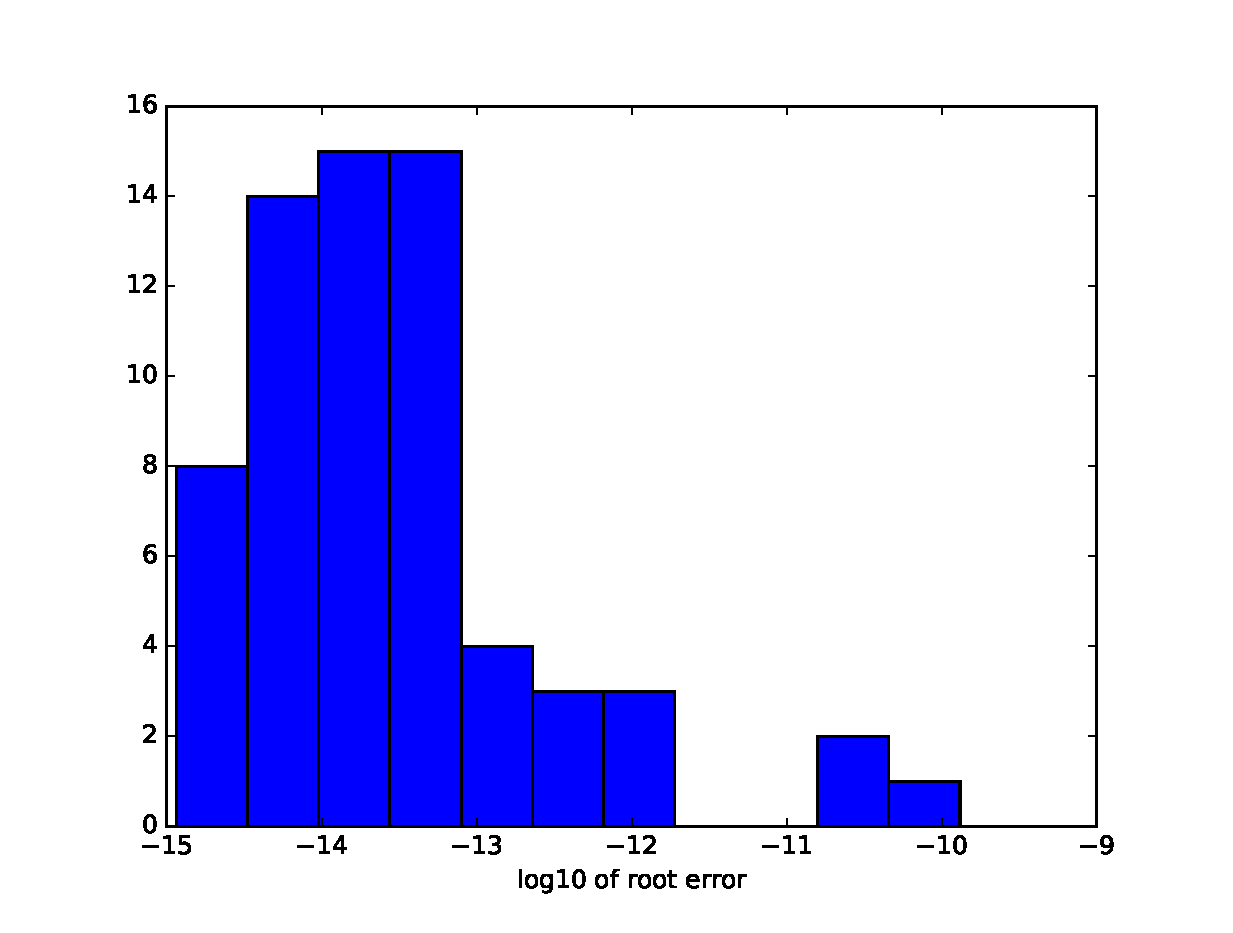
\includegraphics[scale=0.5]{txt/histo_roots.eps}
\end{figure}
\fi

\documentclass{standalone}
% Preamble
\begin{document}

  \begin{thebibliography}{00}

  \bibitem{AS}
  {W. Auzinger, H. J. Stetter},
  {An elimination algorithm for the computation of all zeros of a system of multivariate polynomial equation},
  {Numerical mathematics, Singapore 1998, ISNM vol. 86, Birkhäuser, pp. 11-30}

  \bibitem{Barnett}
  {S. Barnett}, {A note on the Bezoutian matrix},
  {SIAM J. Appl. Math., 22:84-86}, {1972}

  \bibitem{Golub}
  {G.H. Golub, C.F. van Loan},
  {Matrix Computations}, {The Johns Hopkins University Press}, {1989}.

  \bibitem{jpc}
  {J.P. Cardinal}, {Dualité et algorithmes itératifs pour la résolution de systèmes polynomiaux}, {Thèse présentée devant l'université de Rennes I}, {1993}.

  \bibitem{bm}
  {B. Mourrain}, {Bezoutian and quotient ring structure},
  {J. of Symbolic Comput., 39:397-415}, {2005}.

  \bibitem{tm}
  {T. Mora}, {Solving polynomial equation systems}, {Cambridge University Press}, {2015}

  \bibitem{clo}
  {D. Cox, J. Little, D. O'Shea},
  {Ideals, Varieties and Algorithms}, {Springer}, {2006}

  \bibitem{jp_code}
  \url{https://github.com/jpcp13/bezout}

  \end{thebibliography}



\end{document}


\end{document}

%%% Local Variables:
%%% mode: latex
%%% TeX-master: t
%%% End:
